\section{Control and Status Register Files}
Hardware designs often have to be configured from outside of the hardware in order to be used properly. These settings need to be stored in the hardware. Furthermore they also need to be accessible to read out the current configuration along with additional status information.\\
For this purpose registers are used, which are called Control and Status Registers (CSR). They are typically accessed via a host interface by the software and are directly connected to the logic of the hardware design (fig.~\ref{fig:csr}).
\begin{figure}[h]
 \centering
 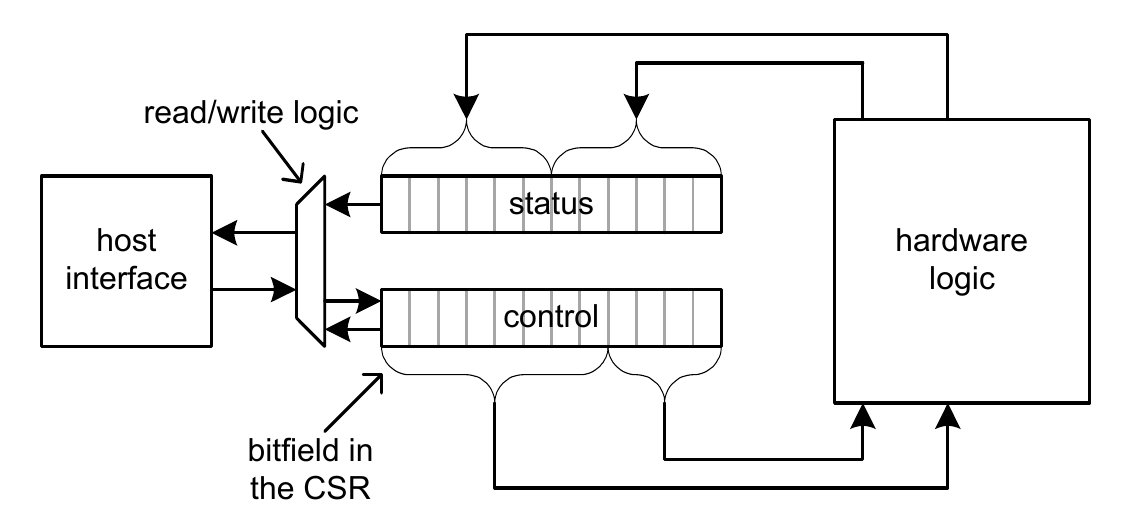
\includegraphics[width=252pt]{images/csr.png}
 \caption{Control and Status Register \cite{leber_diss}}
\label{fig:csr}
\end{figure}

\begin{figure}[h]
 \centering
 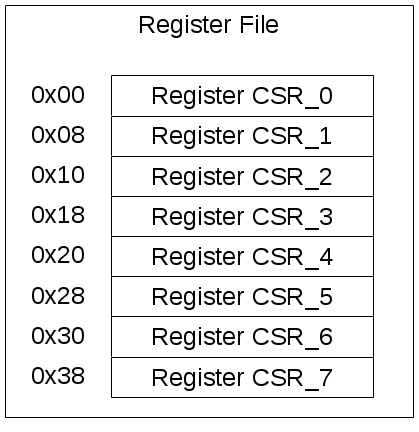
\includegraphics[width=130pt]{images/rf.png}
 \caption{Address Map of a Register File}
\label{fig:rf}
\end{figure}
